\documentclass[journal,12pt,twocolumn]{IEEEtran}
%

\usepackage{setspace}
\usepackage{gensymb}
\singlespacing
\usepackage{hyperref}
\usepackage{amsmath}
\usepackage{amsthm}
\usepackage{txfonts}
\usepackage{cite}
\usepackage{enumitem}
\usepackage{mathtools}
\usepackage{listings}
    \usepackage{color}                                            %%
    \usepackage{array}                                            %%
    \usepackage{longtable}                                        %%
    \usepackage{calc}                                             %%
    \usepackage{multirow}                                         %%
    \usepackage{hhline}                                           %%
    \usepackage{ifthen}                                           %%
  %optionally (for landscape tables embedded in another document): %%
    \usepackage{lscape}     
\usepackage{multicol}
\usepackage{chngcntr}
\renewcommand\thesection{\arabic{section}}
\renewcommand\thesubsection{\thesection.\arabic{subsection}}
\renewcommand\thesubsubsection{\thesubsection.\arabic{subsubsection}}

% correct bad hyphenation here
\hyphenation{op-tical net-works semi-conduc-tor}
\def\inputGnumericTable{}                                 %%

\lstset{
%language=C,
frame=single, 
breaklines=true,
columns=fullflexible
}

\begin{document}
%


\newtheorem{theorem}{Theorem}[section]
\newtheorem{problem}{Problem}
\newtheorem{proposition}{Proposition}[section]
\newtheorem{lemma}{Lemma}[section]
\newtheorem{corollary}[theorem]{Corollary}
\newtheorem{example}{Example}[section]
\newtheorem{definition}[problem]{Definition}
\newcommand{\BEQA}{\begin{eqnarray}}
\newcommand{\EEQA}{\end{eqnarray}}
\newcommand{\define}{\stackrel{\triangle}{=}}
\bibliographystyle{IEEEtran}
\providecommand{\mbf}{\mathbf}
\providecommand{\pr}[1]{\ensuremath{\Pr\left(#1\right)}}
\providecommand{\qfunc}[1]{\ensuremath{Q\left(#1\right)}}
\providecommand{\sbrak}[1]{\ensuremath{{}\left[#1\right]}}
\providecommand{\lsbrak}[1]{\ensuremath{{}\left[#1\right.}}
\providecommand{\rsbrak}[1]{\ensuremath{{}\left.#1\right]}}
\providecommand{\brak}[1]{\ensuremath{\left(#1\right)}}
\providecommand{\lbrak}[1]{\ensuremath{\left(#1\right.}}
\providecommand{\rbrak}[1]{\ensuremath{\left.#1\right)}}
\providecommand{\cbrak}[1]{\ensuremath{\left\{#1\right\}}}
\providecommand{\lcbrak}[1]{\ensuremath{\left\{#1\right.}}
\providecommand{\rcbrak}[1]{\ensuremath{\left.#1\right\}}}
\theoremstyle{remark}
\newtheorem{rem}{Remark}
\newcommand{\sgn}{\mathop{\mathrm{sgn}}}
\providecommand{\abs}[1]{\lvert#1\rvert}
\providecommand{\res}[1]{\Res\displaylimits_{#1}} 
\providecommand{\norm}[1]{\lVert#1\rVert}
\providecommand{\mtx}[1]{\mathbf{#1}}
% \providecommand{\mean}[1]{E\left[ #1 \right]}
\providecommand{\fourier}{\overset{\mathcal{F}}{ \rightleftharpoons}}
\providecommand{\system}{\overset{\mathcal{H}}{ \longleftrightarrow}}
\newcommand{\solution}{\noindent \textbf{Solution: }}
\newcommand{\cosec}{\,\text{cosec}\,}
\providecommand{\dec}[2]{\ensuremath{\overset{#1}{\underset{#2}{\gtrless}}}}
\newcommand{\myvec}[1]{\ensuremath{\begin{pmatrix}#1\end{pmatrix}}}
\newcommand{\cmyvec}[1]{\ensuremath{\begin{pmatrix*}[c]#1\end{pmatrix*}}}
\newcommand{\mydet}[1]{\ensuremath{\begin{vmatrix}#1\end{vmatrix}}}
\newcommand{\proj}[2]{\textbf{proj}_{\vec{#1}}\vec{#2}}
\newcommand{\RNum}[1]{\uppercase\expandafter{\romannumeral #1\relax}}
\let\StandardTheFigure\thefigure
\let\vec\mathbf
\title{
Assignment - 1
}
\author{ Shubham Ramesh Dangat \\SM21MTECH14003}
\maketitle
\newpage
\bigskip
\bibliographystyle{IEEEtran}

\section*{\textbf{Problem}}
\textbf{\textsl{1. The co-ordinates of points A,B are (r_1,$\theta_1$) , (r_2,$\theta_2$) referred to O as pole. The internal bisector of angle AOB meets the line AB in D. Find the co-ordinates of D.}}
\noindent
\section*{\textbf{Solution}}
\textsl{Let the co-ordinates of point D be \myvec{r\\ \theta}.}

\textsl{}

Now , \theta = \dfrac{\theta_1+\theta_2}{2}

\textsl{}

$\therefore$ 
\noindent Converting into rectangular coordinates,

\textsl{}
\begin{align}
\vec{A} = \myvec{r_1sin(\theta_1)\\r_1cos(\theta_1)}, \vec{B} =\myvec{r_2sin(\theta_2)\\r_2cos(\theta_2)},
\end{align}
\begin{align}
\vec{O} =\myvec{0sin(0)\\0cos(0)}, \vec{D} =\myvec{rsin(\theta)\\rcos(\theta)}
\end{align}

For two vectors,
\begin{align}
\vec{a}=\myvec{a_1\\a_2} , \vec{b}=\myvec{b_1\\b_2}
\end{align}
\begin{equation}
\norm{\mathbf{\vec{a}\times\vec{b}}}=\abs{(a_1b_2-a_2b_1)}
\label{eq:2}
\end{equation}
\begin{align}

\vec{A-0}=\myvec{r_1sin(\theta_1)\\r_1cos(\theta_1)},
\vec{A-D}=\myvec{r_1sin(\theta_1)-rsin(\theta)\\r_1cos(\theta_1)-rcos(\theta)}

\textsl{}

\vec{B-D}=\myvec{r_2sin(\theta_2)-rsin(\theta)\\r_2sin(\theta_2)-rcos(\theta)},
\vec{B-O}=\myvec{r_2sin(\theta_2)\\r_2cos(\theta_2)}

\vec{A-B}=\myvec{{r_1sin(\theta_1)-r_2sin(\theta_2)\\r_1cos(\theta_1)-r_2cos(\theta_2)}}

\end{align}
\textsl{}

Since , 

Area (\triangle AOD)+ Area (\triangle DOB) = Area (\triangle AOB)

\textsl{}

\dfrac{1}{2}\norm{\mathbf{(\vec{A}-\vec{O})\times(\vec{A}-\vec{D})}}+\dfrac{1}{2}\norm{\mathbf{(\vec{B}-\vec{D})\times(\vec{B}-\vec{O})}}=

\begin{equation}
\dfrac{1}{2}\norm{\mathbf{(\vec{A}-\vec{O})\times(\vec{A}-\vec{B})}}
\end{equation} 

\textsl{}

$\therefore $ Substituting A-0 , A-D , B-D , B-O , A-B and simplifying further we get,

\textsl{ }

\dfrac{1}{2}\norm{(r_1)\times(r\times sin(\dfrac{\theta}{2}))}+\frac{1}{2}\norm{\mathbfnorm{(r_2)\times(r\times sin(\dfrac{\theta}{2}))}}}


\begin{equation}
= \dfrac{1}{2}\norm{(r_1)\times(r_2\times sin(\dfrac{\theta}{2}))}
\end{equation} \quad

\textsl{}

\textsl{Now , R.H.S = \dfrac{1}{2}\norm{(r_1)\times (r_2 \times sin(\theta))}}

\textsl{}
\begin{equation}
= \dfrac{1}{2}\norm{(r_1) \times (r_2 \times 2 \times sin(\dfrac{\theta}{2}) \times cos(\dfrac{\theta}{2})}}
\end{equation}
\textsl{}

\textsl{On Comparing (6) and (7),}
\textsl{}
\begin{equation}

$\therefore$  \dfrac{1}{2}$\times \norm {r \times (r_1 + r_2)} = \norm{r_1 \times r_2 \times \cos(\dfrac{\theta}{2})}\qquad
\end{equation}
\textsl{ }

\textsl{ }

$\therefore$
\begin{equation}
 r = \abs{(\dfrac{2 \times r_1 \times r_2}{r_1+r_2}\times cos(\dfrac{\theta}{2}))}
\end{equation}

\textsl{ }

\textsl{Now , D has co-ordinates as \mathbf{\myvec{r\\ \theta}}}

\textsl{ }

\textsl{$\therefore$ Co-ordinates of D are \myvec{\dfrac{2 \tmess r_1 \times r_2}{r_1+r_2} \times cos(\dfrac{\theta}{2}) \\ \dfrac{\theta_1+\theta_2}{2}}}

\begin{figure}[!ht]
    \center
    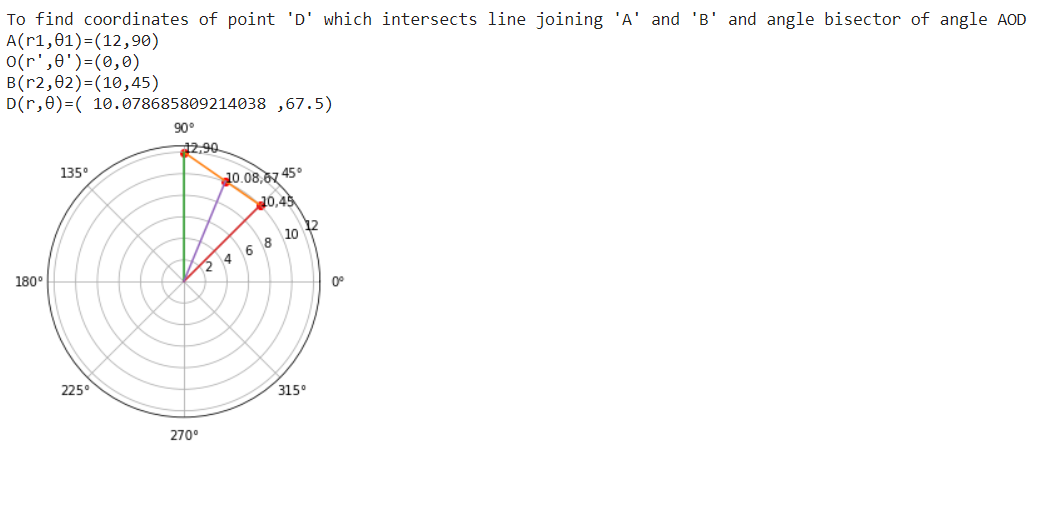
\includegraphics[width=\columnwidth]{BoP_assignment_1.PNG}
    \caption{Triangles AOB,AOD,DOB}
    \label{fig:Quad PQRS}
\end{figure}
\end{document}